\documentclass[manual-fr.tex]{subfiles}
\begin{document}

Pour annoter des documents avec le nouveau modèle, il faut alors sélectionner la chaîne de prétraitement «~NER-retrained.xml~» puis cliquer sur le bouton «~launch SEM~» comme illustré dans la figure \ref{fig:train_sem-07}. Une fois le traitement effectué, SEM indiquera où trouver les fichiers annotés comme illustré dans la figure \ref{fig:train_sem-08}.
To annotate documents with a new model, you need to select the workflow called \emph{NER-retrained.xml} then click on the button \emph{launch SEM} as illustrated in figure \ref{fig:train_sem-07}. Once the processing is done, \SEM\ will tell where to find the newly annotated files as shown in figure \ref{fig:train_sem-08}.

\begin{figure}[ht!]
    \begin{center}
    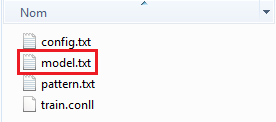
\includegraphics[scale=0.5]{fr/images/train_sem-07.png}
    \end{center}
    \caption{framed in red: the model file to copy in the folder \$\{SEM\_DATA\}/resources/models/fr/NER}
    \label{fig:train_sem-07}
\end{figure}

\begin{figure}[ht!]
    \begin{center}
    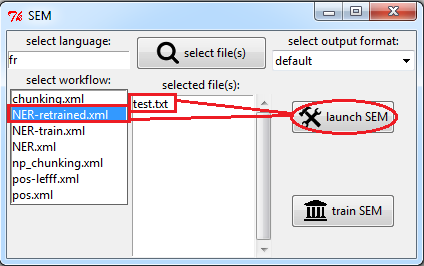
\includegraphics[scale=0.5]{fr/images/train_sem-08.png}
    \end{center}
    \caption{framed in red : the workflow and the file to annotate. Circled in red : the button to launch \SEM.}
    \label{fig:train_sem-08}
\end{figure}

\end{document}
